\chapter{Deep Learning in Digital Histopathology}

We begin by introducing the field of histopathology and its concerns alongside tools and methods used in contemporary clinical practice.
We show how digitization helped to reduce the logistical complexity of histopathologists' workflow and how decision support systems can further reduce the required human labor.
We introduce feedforward artificial neural networks, later focusing on convolutional networks, which are exceptional at tackling various computer vision problems.

\section{Histopathology}

Histopathology is a discipline concerned with the study of diseases of tissue.
Scope of histopathology involves, but is not limited to, cancer detection and prediction, infectious or inflammatory disease diagnostics, and the study of brain-degenerative diseases such as Parkinson's or Alzheimer's \cite{histopathology-cancer, histopathology-infectious, histopathology-inflammatory, histopathology-brain-degenerative}.

Royal College of Pathology in \cite{histopathologist-role} defines histopathologists as medically qualified physicians who inspect patient tissue samples.
Their expertise is essential in identifying cellular and tissue anomalies that could indicate various medical conditions.
Histopathologists often cooperate with other doctors, providing insights to help set the direction of further patient care.

\section{Temporal and Spatial Limitations of Traditional Histopathology}

Traditionally, a tedious logistic process involving several people is necessary to get tissue from a patient to a histopathologist.
The surgeon needs to extract tissue samples from the patient.
A specialized laboratory then receives the extracted tissue for processing; technicians infuse the tissue samples with a mix of chemicals and embed them into a paraffin wax block.
The paraffin block is then thinly sliced into thin sections, and technicians laminate those sections onto a glass slide.
Glass slides are stained with hematoxylin/eosin (or another compound, depending on the use case, as per \cite{histopathology-staining}) to enhance the contrast between different cellular structures.
After the lab processing, slides are delivered to a histopathologist for review \cite{histo-process}.

While we cannot replace the surgeons performing the biopsy or lab workers staining and embedding the tissue, we can address the logistic challenges of moving glass slides to the histopathologists.
Having a physical slide suffers from several inefficiencies. 
Only one histopathologist can study a slide at a time. If a second opinion from a different histopathologist is required, a designated person must convey the glass slide to the respective clinic.
Such logistic pitfalls throttle the diagnosis process and lead to longer waiting times for a patient \cite{from-traditional-to-digital-histopathology}.

\section{Digital Histopathology}
% https://pathsocjournals.onlinelibrary.wiley.com/doi/10.1002/path.5388

Digital histopathology aims to reduce the logistic overhead caused by physical copies of glass slides.
After the tissue is extracted and prepared, instead of shipping it to a histopathologist, it is scanned using specialized lenses, resulting in a high-resolution digital image called \emph{Whole Slide Image} (WSI) \cite{from-traditional-to-digital-histopathology}.
This image is then uploaded to an aggregator server, enabling real-time slide sharing and parallel cooperation of multiple clinicians.
Histopathologists then inspect WSI's in a dedicated browser on their computer monitors --- opposed to looking at the glass slide under a microscope \cite{digital-histopathology-process}. \myref{Figure}{fig:xopat} shows a WSI of prostate tissue sample displayed in a dedicated browser developed by the RationAI group.

Even though contemporary digital pathology systems significantly speed up pathologists' day-to-day work, we can further optimize another productivity metric: pathologists' time spent inspecting WSIs.

\begin{figure}
    \begin{center}
    \begin{minipage}{0.80\textwidth}
      \fcolorbox{RoyalBlue}{white}{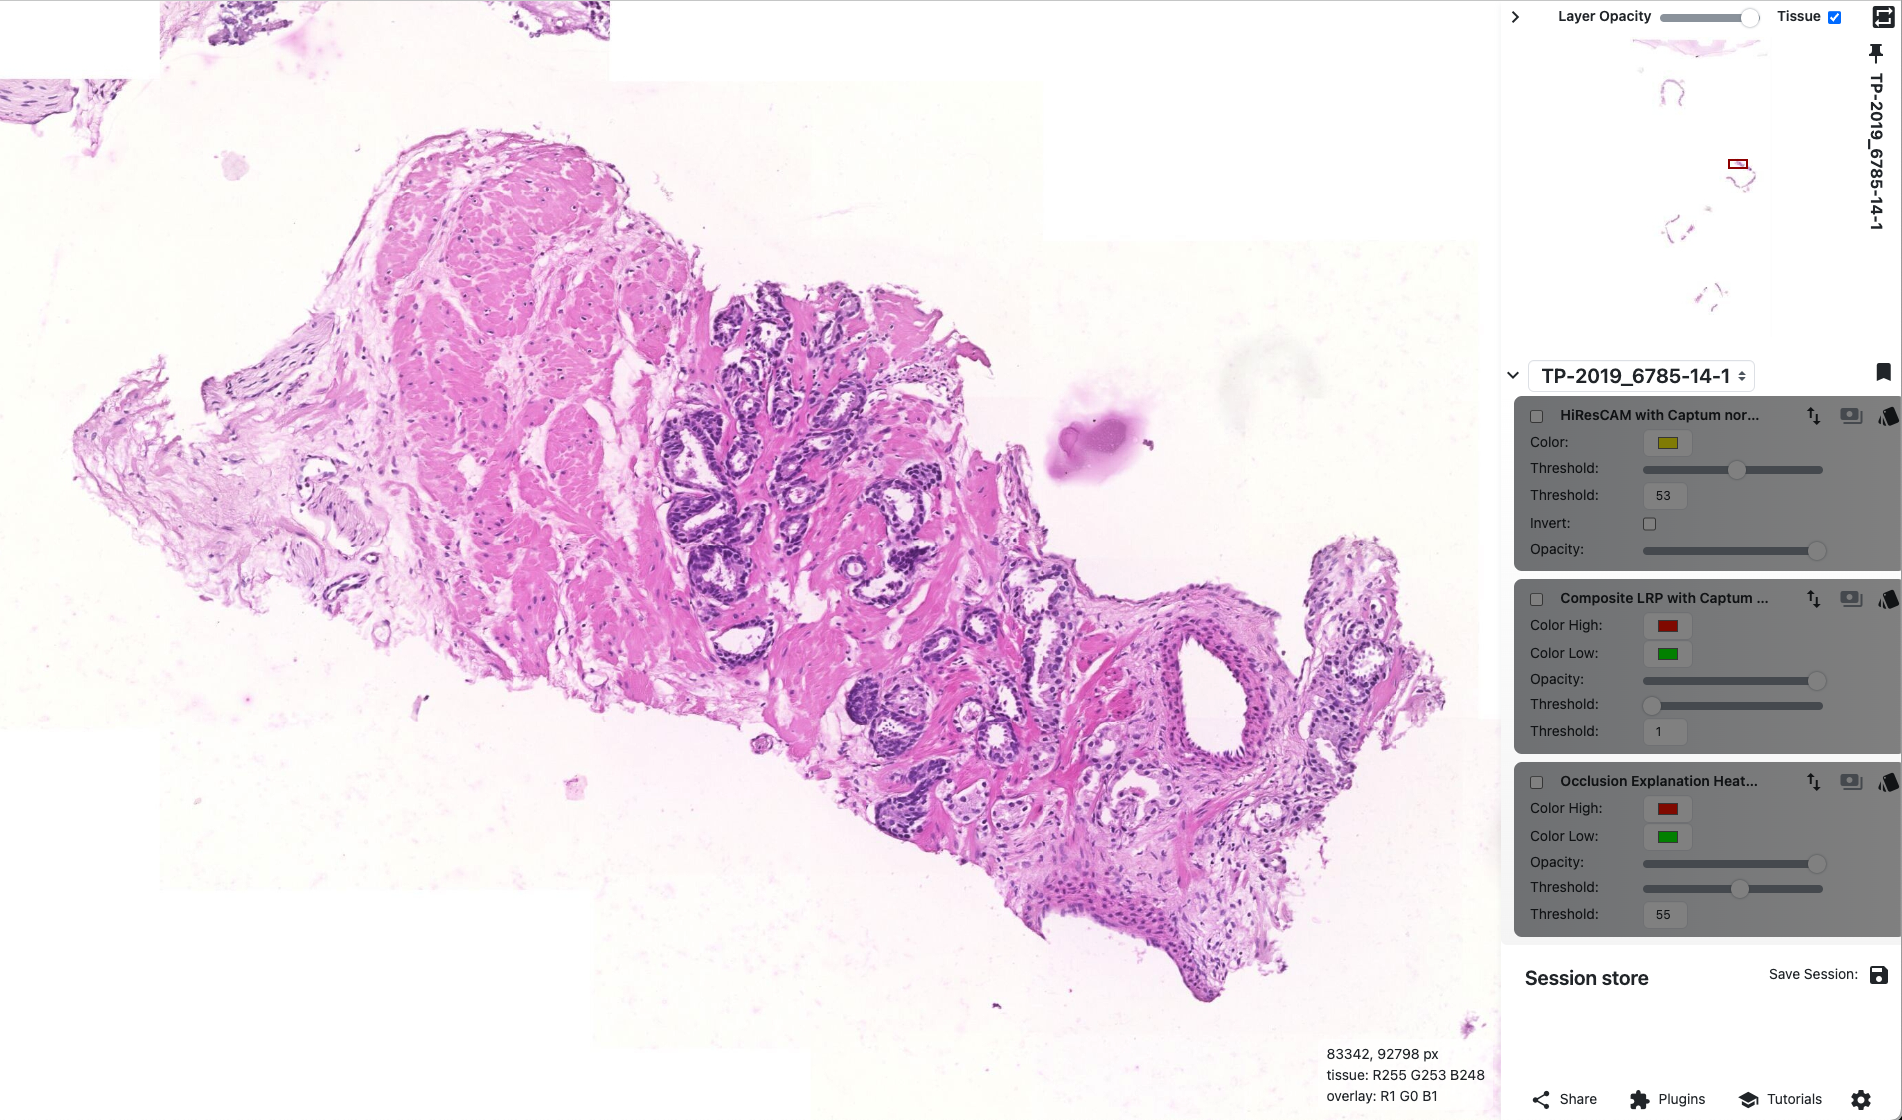
\includegraphics[width=\textwidth]{img/xopat.png}}
    \end{minipage}
    \caption{xOpat \cite{xopat} WSI browser with a sample of prostate tissue. The histopathologist can move and zoom the tissue, allowing him to navigate the WSI quickly. Digitized copies allow for the layering of arbitrary annotations on top of the WSI, providing great collaborative capabilities. Different pathologists can mark cancerous regions and then display them on top of each other to see their agreement.}
    \label{fig:xopat}
    \end{center}
\end{figure}

\subsection*{Decision Support System}

A computer system that aids humans in deciding while performing a particular task is called a decision support system.
These systems are utilized across various applications, including high-stake environments such as investment banking, autonomous driving, or military and defense \cite{dss-finance, dss-autonomous-driving, dss-military-and-defense}. In digital histopathology, clinicians usually utilize such systems to help with operational processes \cite{digital-histopathology-process}.
However, with deep learning in the spotlight of today's research, new possibilities emerge.

Systems based on deep learning could enhance the tissue diagnostic process by assisting diagnosis or discovering previously unrecognized features in large sets of data that are incomprehensible to a single expert \cite{dss-digital-histopathology}. 
Researchers and various companies are actively trying to employ machine learning systems in such a fashion. 
Those systems often provide real-time results and domain-expert-like performance, demonstrating that further research can significantly improve contemporary processes \cite{deep-learning-in-histopathology}.

\section{Deep Learning}\label{section:dl}

The area of machine learning encapsulating neural networks (NNs) is called deep learning (DL).
Methods and algorithms employed by DL achieve remarkable results across various domains, including computer vision, games, or weather forecast \cite{alexnet, alphago, weather}.
Introduced by McCulloch and Pitts in \cite{mcculloch-pitts} to create a computational unit resembling a neuron in the human brain, neural networks have come a long way to the prominent place they occupy today.

\subsection*{Feedforward Neural Network}\label{feedforward-nn}

Feedforward networks are considered the starting point of contemporary DL models.
They get their name from a one-directional flow of information inside the network.
We can see feedforward networks as a function $f$ that maps real-valued input vector $x$ from input space to a value $y$ from output space \cite{goodfellow}.
Throughout this thesis, we will only consider this type of network.

A common approach to examining neural network architectures is to see them as a sequence of layers.
Each layer $l$ resembles an intermediate function $f^l$.
Let our network be a composition of $L$ layers numbered from $1$ to $L$.
For any given input vector $x$, the computation performed by the network can be expressed as a composition of its intermediate layer functions, yielding
\begin{equation}
    f(x) = f^L(f^{L-1}(\cdots f^1(x))).
\end{equation}
In this notation, layer $1$ is the input layer, which receives the input vector $x$. The final or $L$-th layer is the output layer, which returns the network's prediction or decision $y$. All in-between layers are called hidden layers and transform one internal representation to another \cite{goodfellow}.

Even though \cite{cybenko} essentially shows that one hidden layer is all you need, neural networks typically employ multiple hidden layers.
The motivation is that we can see each layer as if it captures specific abstractions or representations from its input.
Deeper layers can, therefore, build more complex representations by utilizing abstractions captured by previous layers.

Multi-layer Perceptron (MLP) is a foundational architecture in the history of feedforward neural networks.
In an MLP, the basic building block is a neuron.
Neurons are arranged into layers to form the final network.
A neuron receives input signals (input features $x$), processes them, and outputs its signal ($y$), which is passed to subsequent neurons in the following layer.
The processing consists of computing inner potential $\xi$, a weighted average of the neuron's inputs.
The inner potential is then passed to the activation function, denoted as $\sigma$. 
% \footnote{Heaviside step function was the first activation function used. This led to several problems [], and activation functions are a vital part of contemporary because of their importance.}, 
Given a neuron $i$ with activation function $\sigma_i$ expecting $K$ input signals, the output signal $y_i$ is expressed as
\begin{equation}
    y_i = \sigma_i(b_i + \sum_{k=1}^K w_{ik}x_k)
\end{equation}
where weight $w_{ik}$ connects $k$-th input feature to the neuron $i$ and $b_i$ is a constant bias term, improving the neuron's modeling capabilities.
If all neurons in a given layer $l$ have incoming weights from all neurons in the previous layer, we say that $l$ is fully connected (FC) \cite{goodfellow}.
% \myref{Figure}{fig:simple-mlp} depicts a small MLP with one hidden layer.

Weights and biases are called trainable parameters, denoted as $\theta$.
Deep learning aims to make the trainable parameters useful.
Since a network computes a function $f$, with specific training, we can make the network configure its parameters to approximate a desired function $f^*$ within a certain tolerance.
To configure the parameters, we leverage a large amount of data to minimize the difference between $f$ and $f^*$.
The difference is captured using loss function $\ell$, and minimizing $\ell$ is typically performed iteratively using backpropagation and training algorithms such as stochastic gradient descent.
More on neural network training can be found in \cite{goodfellow}.

% Although a deep dive into training is out of the scope of this thesis, we need to familiarize ourselves with the notion of partial derivatives.
% Partial derivatives are commonly used to find a direction against which we move certain weight $w$ to minimize the $\ell$ if all other parameters remain fixed.
% We denote the partial derivative of $\ell$ with respect to parameter $w$ as $\frac{\partial \ell}{\partial w}$.
% Building on the concept of partial derivatives, we can compute the gradient.
% In the context of a deep learning model's loss function, the gradient $\nabla_{\theta}\ell$ is a vector of partial derivatives of $\ell$ with respect to all the parameters within the model
% \begin{equation}
%     \nabla_{\theta}\ell = \left( \frac{\partial \ell}{\partial w_1}, \frac{\partial \ell}{\partial w_2}, \cdots, \frac{\partial \ell}{\partial w_{|\theta|}} \right).
% \end{equation}
% This gradient points in the direction of the steepest ascent in the loss function's value.
% Thus, to minimize, we update the parameters in the opposite direction of the gradient.
% As we will see in Chapter 3, partial derivatives can also be leveraged to compute importance of features or networks parameters.
% \todo{ref}
% %% goodfellow kniha

% \begin{figure}
%     \begin{center}
%     \begin{minipage}{.75\textwidth}
%       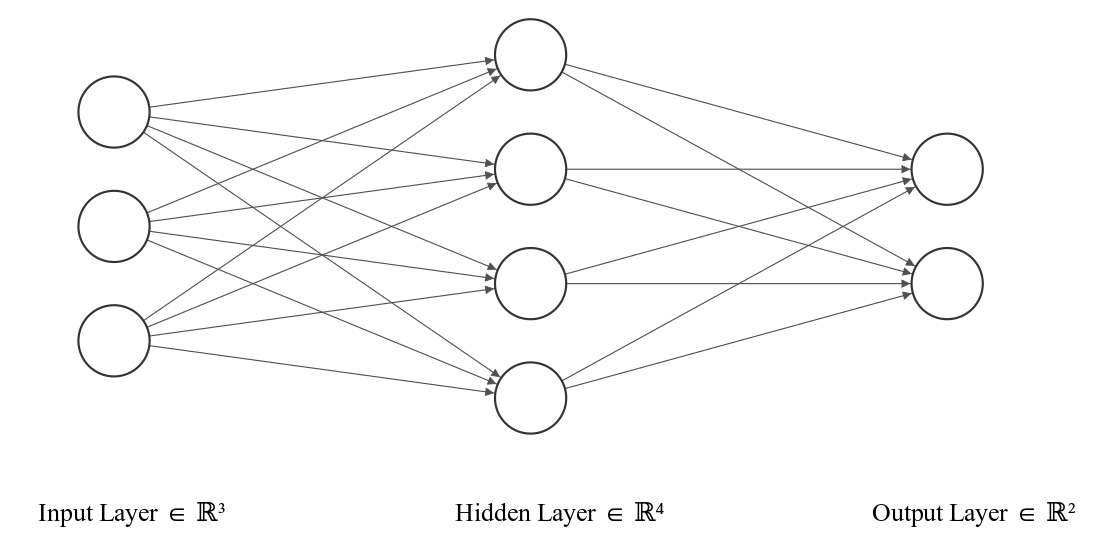
\includegraphics[width=\textwidth]{img/nn.png}
%     \end{minipage}
%     \caption{Architecture of an MLP with one hidden layer. Circles represent layer neurons. Edges represent layer weights. Biases are omitted for simplicity. Notice that each neuron in the hidden and output layer shares weight with all neurons in the previous layer -- therefore, layers are fully connected.}
%     \label{fig:simple-mlp}
%     \end{center}
% \end{figure}

Even though MLPs demonstrate impressive results on tasks previously deemed impossible for computers, they come with certain setbacks.
If we only use FC layers, contemporary architectures such as AlexNet \cite{alexnet} would have an unimaginable number of trainable parameters.
This led to the development of new architectures tailored to specific domain needs.
Despite the shift from using FC layers only, MLP stood its ground and, to this day, is an essential part of various state-of-the-art neural network architectures \cite{alexnet}.

\subsection*{Convolutional Neural Network}
Convolutional neural networks (CNNs) focus on working with grid-like data.
Therefore, their input $x$ typically comes in the form of a multidimensional array of shape $H \times W \times C$, where $H$ and $W$ stand for height and width respectively, and $C$ is the number of channels ($1$ for grayscale images, $3$ for RGB images).
CNNs were introduced specifically to solve various computer vision problems and add two additional layer types --- convolutional and pooling.
These layers help to capture patterns in input features, as well as reduce the size of the network \cite{cnns}. 
%% - https://arxiv.org/pdf/1511.08458.pdf

%% TODO: Why it suits them for image processing

\subsubsection{Convolutional Layer}

The convolutional layer utilizes trainable filters (kernels) to search for visual patterns in its features.
The filter is typically smaller in width and height than the input but spans all the input channels.
Instead of interacting with the whole input at once using weighted connections, the filter $F$ is systematically slid across the input, and the filter weights convolve with the corresponding input data segments, yielding a two-dimensional \emph{activation map} $A$ \cite{goodfellow}.
Convolution is a linear operation that chains the element-wise product of the filter and receptive field over all channels and then sums the products into one value. Given a filter $F$ and input $I$, spatial activation $A_{ij}$ is computed as 
\begin{equation}
    (F * I)_{ij} = b + \sum_{x=0}^{W} \sum_{y=0}^{H} \sum_{z=0}^{C} F_{xyz} \cdot I_{(i+x)(j+y)z}
\end{equation}
where $W$, $H$ are width and height of $F$ and $C$ is number of input channels. The bias term $b$ is used similarly as in the case of fully connected layers.

The resulting activation map can be seen as a map of evidence for the presence of a shape detected by the filter in the input data.
Sliding the filter through features gives us spatial invariance --- no matter where the learned pattern resides in the input, it will be detected and reflected in the respective activation map, something very hard to achieve using a fully connected layer.
Therefore, we commonly say that the filter has \emph{shared weights} \cite{goodfellow}.

When incorporating a convolutional layer into a neural network, the crucial parameter to define is the filters' shape.
The shape determines the receptive field's size -- how many input features the filter can see at one given position.
In addition, we usually set two other parameters: \emph{padding} and \emph{stride}.
Padding is a value we add as a border around the input features, allowing the filter to cover the edges and thus reducing information loss.
Stride controls how much we shift the filter after each convolution \cite{cnns}.

% \begin{figure}
%     \begin{center}
%     \begin{minipage}{0.75\textwidth}
%       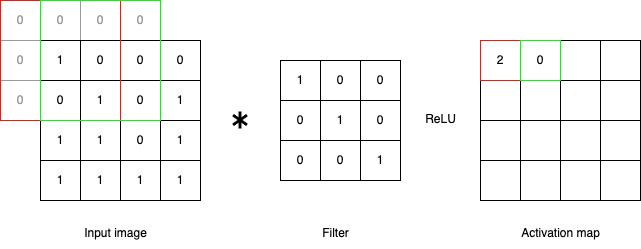
\includegraphics[width=\textwidth]{img/cnn-conv.png}
%     \end{minipage}
%     \caption{Example of simple calculation within convolution layer. The filter detects a diagonal edge of 3 pixels in length. Stride and padding are set to $1$ pixel, and zero is used as the padded value. We omit the bias term from the calculation. The result is passed through the ReLU activation function.}
%     \label{fig:cnn-convolution}
%     \end{center}
% \end{figure}

A convolutional layer consists of multiple units.
Each unit has its filter and produces a unique activation map.
The idea is that each filter learns to recognize a different pattern during training --- and each unit is a map of evidence of those patterns.
This gives a single layer the capability to detect multiple patterns, and, similarly to its fully connected counterpart, it allows subsequent layers of the network to build upon captured abstractions and ultimately "understand" and represent high-level concepts.
Given a layer with $n$ units, we will denote $k$-th filter as $F^k$ and $k$-th activation map as $A^k$.

It is important to note that sharing weights has not only effects of identifying patterns regardless of their position in the input -- it also reduces the number of parameters we have in a network \cite{cnns}.

\subsubsection{Pooling Layer}

To prevent overfitting, pooling layers are employed to additionally distill captured patterns.
They progressively reduce the size of the input features, leading to a smaller number of model parameters and reduced computational time \cite{cnns}.

A pooling layer is typically placed after a convolutional one, iterating its activation maps and systematically applying a specific operation over its receptive field.
We differentiate between two primary types of pooling: \emph{max} and \emph{average}.
As their names imply, max pooling selects the maximum value within its receptive field, while average pooling computes the mean of the values.
% The pooling layer has its shape and stride.
% However, the dimensions are chosen more conservatively.
% A common choice is a $2 \times 2$ filter and stride of $2$, ensuring the pooled sectors do not overlap.
% According to the observations in \cite{cnns}, having a filter of size greater than $3 \times 3$ will most likely lead to a loss of the model's performance --- since such granularity may hide too many of the features detected by the network.
% 
% \begin{figure}
%     \begin{center}
%     \begin{minipage}{0.5\textwidth}
%       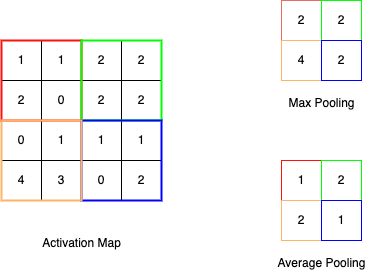
\includegraphics[width=\textwidth]{img/cnn-pool.png}
%     \end{minipage}
%     \caption{Example of both max and average pooling layers. Both have filters of size $2x2$ and stride set to $2$, resulting in no overlap during computation. Notice that since each $2x2$ region is mapped to a single value, the new activation mask has a quarter of the features of the original.}
%     \label{fig:cnn-pooling}
%     \end{center}
% \end{figure}

\subsubsection{Global Pooling Layer}

Given that our network comprises only convolutional and pooling layers, we are not bound to any specific input size.
Nonetheless, it is common practice to introduce fully connected layers towards the end of the network, and they require a fixed-size number of input features \cite{cnns}.
To meet this requirement, we use global pooling layers.

Like standard pooling, global pooling comes in two forms: max and average.
The global pooling layer condenses each activation map into a single value.
This guarantees that if a convolutional layer has $n$ units and the subsequent fully connected layer receives $n$ input features, placing a global pooling layer in between will provide a compatible transition, standardizing the output size of the last convolutional or pooling layer regardless of the original input data dimensions.

Throughout this thesis, we will denote globally pooled activation map $A^k$ as $a^k$. For a global average pooling (GAP) layer, the $a^k$ is computed as
\begin{equation}\label{gap}
    a^k = \frac{1}{|A^k|} \sum_{i=0}^H \sum_{j=0}^W A^k_{ij}
\end{equation}
and for the global max pooling, the \myref{Equation}{gap} changes to simply
\begin{equation}
    a^k = \max_{i,j} A^k_{ij}.
\end{equation}